%Author: Tore Arndt, Patrick Otte
\nsecbegin{Ziel des Sprints}
Es soll eine funktionsfähige Basisversion, welche für das einfache erstellen von Klassendiagrammen aus Java-Code verwendet werden soll entstehen. Das Programm soll sowohl über die Kommandozeile, als auch über eine grafische Oberfläche bedient werden können. Die erzeugten Klassendiagramme sollen in der grafischen Oberfläche angezeigt werden können.

\begin{figure}[hbtp]
\centering
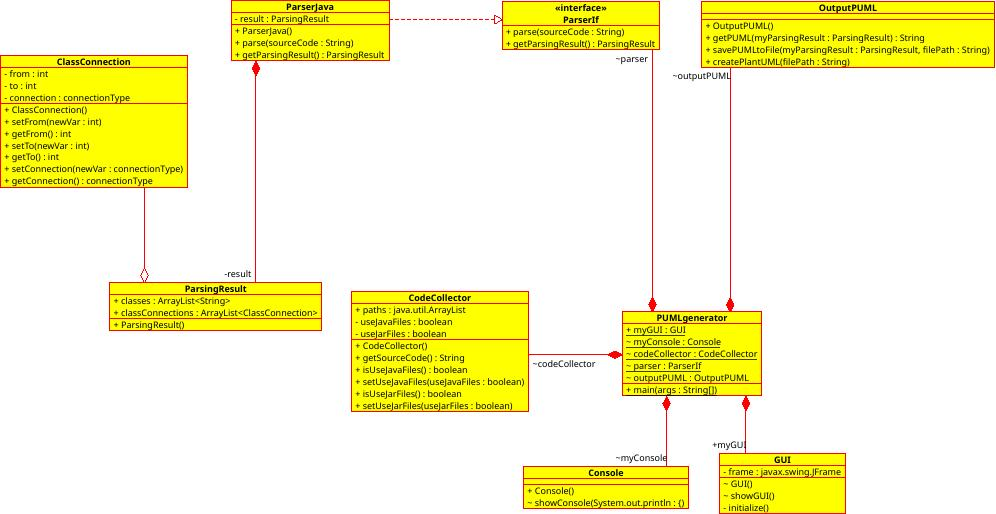
\includegraphics[scale=0.5]{Bilder/classDiagrammSprint1}
\caption{Klassendiagramm des Sprints}
\end{figure}
\nsecend

\nsecbegin{User-Stories des Sprint-Backlogs}
\nsecbegin{Dateien einlesen}
\nsecbegin{Art der eingelesenen Datei}
Als Benutzer wünsche ich mir, dass eine Auswahl zwischen Jar- und Java-Dateien möglich ist, damit Quellcode nicht doppelt eingelesen wird.
\nsecend

\nsecbegin{Java-Dateien}
Als Benutzer wünsche ich mir, dass Java-Dateien einlesbar sind, um den Quellcode von einer oder mehreren Klassen zu analysieren.
\nsecend

\nsecbegin{Jar-Dateien}
Als Benutzer wünsche ich mir, dass Jar-Dateien einlesbar sind, um den Quellcode zu analysieren.
\nsecend
\nsecend

\nsecbegin{Vorschau}
Als Benutzer wünsche ich mir eine Vorschau der Diagramme, damit ich einschätzen kann ob ich damit zufrieden bin.
\nsecend

\nsecbegin{Kommandozeile}
Als Benutzer wünsche ich mir, dass das Programm von der Kommandozeile aus aufrufbar ist, um es automatisiert starten zu können.
\nsecend

\nsecbegin{Klassendiagramme}
Als Benutzer wünsche ich mir, Klassendiagramme aus meinem bestehenden Quellcode erstellen zu können, damit ich das nicht manuell tun muss.
\nsecend

\nsecbegin{Anzeigen und Speichern von PlantUML}
Als Benutzer wünsche ich mir, Diagramme als PlantUML-Code anzeigen und speichern zu können, um den Aufbau nachvollziehen zu können.
\nsecend

\nsecbegin{Plattformunabhängigkeit}
Als Project Owner wünsche ich mir, dass das Programm plattformunabhängig ist, damit es sich gut verbreiten lässt.
\nsecend
\nsecend % {User-Stories des Sprint-Backlogs}

\nsecbegin{Zeitliche Planung}
\begin{figure}[hbtp]
\centering
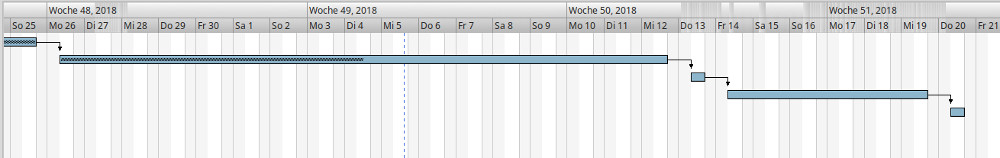
\includegraphics[width=\textwidth]{Bilder/gantt}
\caption{Gantt-Diagramm für Sprint 1}
\end{figure}
\nsecend

\nsecbegin{Liste der durchgeführten Meetings}
\begin{itemize}
\item Planning-Meeting (29.11.2018)
\item Zwischen-Meeting (03.12.2018)
\item Review-Meeting (13.12.2018)
\end{itemize}
\nsecend

\nsecbegin{Ergebnisse des Planning-Meetings}
Dem gesammten Team ist die geplante Grundstruktur des Programms bekannt. Jeder weiß welchen Teil des Programms er implementieren soll.
\nsecend

\nsecbegin{Aufgewendete Arbeitszeit pro Person$+$Arbeitspaket}
\begin{longtable}{|p{4cm}|l|l|l|l|l|}
        \hline
        Arbeitspaket & Person & Start & Ende & h & Artefakt\\
        \hline
        PUML-26/36 & Patrick Otte & 26.11.18 & 21.12.18 & 14 & OutputPUML.java\\ \hline
        PUML-26/37 & Tore Arndt & 26.11.18 & 21.12.18 & 14 & OutputPUML.java\\ \hline
        PUML-24/29 & Leo Rauschke & 26.11.18 & 21.12.18 & 11,5 & CodeCollector.java\\ \hline  
        PUML-24/30 & Elisabeth Schuster & 26.11.18 & 21.12.18 & 11 & CodeCollector.java\\ \hline  
        PUML-25/31 & Jona Meyer & 26.11.18 & 21.12.18 & 30 & Parser.java\\ \hline  
        PUML-24/32 & Michael Lux & 26.11.18 & 21.12.18 & 17 & Parser.java\\ \hline  
        PUML-27/34 & Johann Gerhardt & 26.11.18 & 21.12.18 & 10 & Console.java\\ \hline
        PUML-27/35 & Marian Geißler & 26.11.18 & 21.12.18 & 11 & Console.java\\ \hline
        PUML-28/33 & Jan Sollmann & 26.11.18 & 21.12.18 & 12 & GUI.java\\ \hline
        PUML-28/38 & Julian Uebe & 26.11.18 & 21.12.18 & 14 & GUI.java\\ \hline
\end{longtable}     
\nsecend

\nsecbegin{Konkrete Code-Qualität im Sprint}
Es gibt an vielen Stellen noch erheblichen Optimierungsbedarf. Teils Code doppelt anstatt in Methoden oder durch bessere Struktur nur einmal vorhanden. Des Weiteren fehlen an vielen Stellen Kommentare und Dokumentationen zu den jeweiligen Methoden. Die vorher vom Softwarearchitekten vorgegebenen Coding Conventions und Styles müssen umgesetzt und beachtet werden, sodass, bei einem später geplanten eigenen Merge, Konflikte vermieden werden können.
\nsecend

\nsecbegin{Konkrete Test-Überdeckung im Sprint}
Testüberdeckung liegt bei 41,2\%.
\nsecend

\nsecbegin{Ergebnisse des Reviews}
\begin{table}[H]

\begin{tabularx}{\textwidth}{ |l|l|X| }
\hline
\textbf{Klasse} & \textbf{Methode} & \textbf{Anmerkungen}\\
 \hline
Console & showConsole & Pfad anpassen \\
CodeCollector & - & Unit-Tests für Ordner \\
CodeCollector & getSourceCode & gleichzeitig .jar- und .java-Dateien \\
ParserJava & parse & Bug: Entfernt zu viel Source Code! Mehr Tests\\
OutputPuml & - & generell mehr Kommentare \\
OutputPuml & getPuml & Redundanter Code mit savePumlToFile, generell mehr Kommentare\\
OutputPuml & createPlantUML & Performance verbessern \\
GUI\_SWT & - & Entwicklerdokumentation (Installationsanleitung) für verwendetes Tool\\
\hline
\end{tabularx}
\end{table}

Sonstiges:
\begin{itemize}
\item mehr Kommentare
\item (Graphviz muss installiert sein, um PlantUML anzuzeigen)
\item Javadocs schreiben!
\item in gitconfig Name und Mail-Adresse anpassen! Wichtig für Benotung!
\item Ordner für Unit-Tests ist srcTest
\item im Ordner srcTest ein Unterordner "'testfiles"' ertellen, in dem zusätzliche Testdateien landen
\end{itemize}
\nsecend

\nsecbegin{Ergebnisse der Retrospektive}
\begin{figure}[hbtp]
\centering
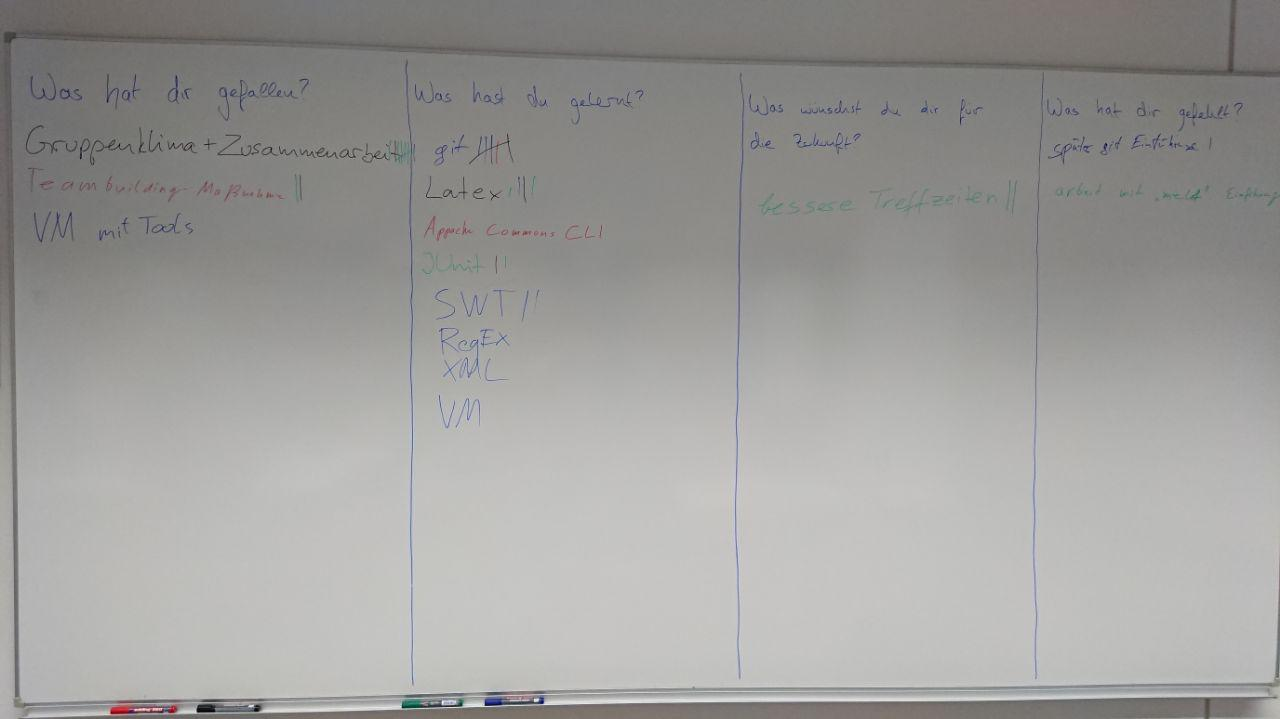
\includegraphics[scale=0.4]{Bilder/Retrospektive_Tafelbild.jpg} 
\caption{Anmerkungen der Teammitglieder zum bisherigen Verlauf des Projekts}
\end{figure}
Die Retrospektive schloss, sowohl was den Lernerfolg als auch die Kommunikation im Team angeht, mit einer positiven Bilanz. Gelobt wurde besonders das Gruppenklima und die Zusammenarbeit sowie die Verteilung der fertig eingerichteten Virtual Machine. Kollektive Lernerfolge sind besonders in den Bereichen Git und Latex zu verzeichnen, daneben decken die genannten spezialisierten Bereiche die Themenfelder ab, die den jeweiligen Gruppen zugeteilt wurden. Für die Zukunft hofft das Team auf günstigere Zeiten für die Projekttreffen. Bemängelt wurde, dass es bei der Einführung in das Arbeiten mit Git allgemein Defizite gab. Spezifisch machte besonders die Bedienung des Meld-Tools Schwierigkeiten. Es wurde deshalb beschlossen, auf diese Probleme in einem der folgenden Gruppentreffen noch einmal ausführlich einzugehen.\\
Befürchtet wurde vor allen Dingen, dass im nächsten Semester mehr Fehler auftreten werden, als das Team zunächst vermutet hätte. Um das Risiko zu verringern, dass sich diese Befürchtungen bewahrheiten, wurden bereits bekannte Bugs zusammengetragen und in Jira gestellt. Ziel des zweiten Sprints ist die vollständige Implementierung aller für den ersten Sprint definierten Use Cases (sofern noch nicht erfolgt) wie auch das Beheben aller bisher dokumentierten Bugs. Die Praxis des Pair Programmings wird zunächst beibehalten. Angestrebt ist dennoch eine bessere Dokumentierung des Quellcodes, auch, um eine potenzielle Umverteilung der Teammitglieder zu erleichtern. Im nächsten Semester soll für die Teammitglieder die Möglichkeit bestehen, auf Wunsch in einen anderen Teilbereich des Projektes \glqq hineinzuschnuppern\grqq. Auch die in Jira angelegten Issues sollen besser getrennt werden, um sie auch an Einzelpersonen zuweisen zu können.\\ \\
\nsecend

\nsecbegin{Abschließende Einschätzung des Product-Owners}
Insgesamt konnten die meisten für den ersten Sprint definierten Use Cases implementiert werden. Damit existiert bereits eine minimale, lauffähige Version des Programms. Werden im nächsten Sprint die noch nicht vollständig im ersten Sprint implementierten Funktionen fertiggestellt sowie enthaltene Bugs entfernt, ist eine solide Grundlage für die weitere Entwicklung des Produkts gelegt.
\nsecend

\nsecbegin{Abschließende Einschätzung des Software-Architekten}
Die elementarsten Funktionalitäten sind implementiert. Die für die Architektur entworfenen Schnittstellen greifen wie geplant ineinander. 
\nsecend

\nsecbegin{Abschließende Einschätzung des Team-Managers}
Für dieses Projektteam ist die Rolle des Team-Managers nicht vergeben. Von den Ergebnissen der Retrospektive ausgehend lässt sich allerdings annehmen, dass die bisherige Vorgehensweise bei der Organisation des Projekts sowie der Durchführung der Treffen und des ersten Sprints grundsätzlich ein guter Ansatz zu sein scheint. 
\nsecend

